\documentclass[a4paper,11pt]{article}
%@@@@@@@@@@@@@@@@@@@@@@@@@@@@@@@@@@@@@@@@@@@@@@@@@@@@@@@@@@@
%@@@@@@@@@@@@@@@@      PACOTES BÁSICOS		     @@@@@@@@@@
%@@@@@@@@@@@@@@@@@@@@@@@@@@@@@@@@@@@@@@@@@@@@@@@@@@@@@@@@@@@

\usepackage[T1]{fontenc}
\usepackage[utf8]{inputenc}
\usepackage{lmodern} 
\usepackage[portuguese]{babel}
\usepackage{amsmath}
\usepackage{array}
\usepackage{graphicx}				%para imagens
\usepackage{epstopdf} 				%resolve problemas eps-pdf
\usepackage{pict2e}				%%writting to images
%@@@@@@@@@@@@@@@@@@@@@@@@@@@@@@@@@@@@@@@@@@@@@@@@@@@@@@@@@@@
%@@@@@@@@@@@@@@@@     PACOTES NÃO TAOBÁSICOS		 @@@@@@@@@@
%@@@@@@@@@@@@@@@@@@@@@@@@@@@@@@@@@@@@@@@@@@@@@@@@@@@@@@@@@@@
\usepackage{fancyhdr}				% para o cabeçalho bonito
\usepackage{caption}					%para legendas
\usepackage{subcaption}				% e sublegendas
\usepackage{placeins} 				%controlar o lugar dos floats
\pagestyle{fancy} 					% número de pag e cabeçalho
\usepackage{txfonts} 				%fontes bonitas? acho que para o título
\usepackage[usenames]{color} 		% algo com gunplot e eps
\usepackage{ifthen}
\usepackage{xparse}
\graphicspath{{./../images/}{./../data/}{./graph/}}	% procura imagens nessa pasta
\usepackage{float} %%para definir ambiente gráfico
\newfloat{Gráfico}{hbtp}{lop}[section]
%\usepackage{undertilde}	%%para notação de vetor do yuri
\usepackage[import]{xy} % para escrever em imagens
\xyoption{import}

\usepackage{listings}
\lstset{frame=single,}
%@@@@@@@@@@@@@@@@@@@@@@@@@@@@@@@@@@@@@@@@@@@@@@@@@@@@@@@@@@@
%@@@@@@@@@@@@@@@@      Cabeçalho de cada página      @@@@@@@
%@@@@@@@@@@@@@@@@@@@@@@@@@@@@@@@@@@@@@@@@@@@@@@@@@@@@@@@@@@@
\setlength{\headheight}{25pt}%compila sem erro
	\fancyhead{}
	\fancyfoot{}
	\fancyhead[R]{Sistemas de Medição}%direito superior
	\fancyhead[L]{
\includegraphics[height=0.25in]{./../images/logo_unb.pdf}}%esquerda superior
	\fancyfoot[C]{\thepage}%baixo centro
%E: Even page, O: Odd page, L: Left field, C: Center field, R: Right field, H: Header, F: Footer
% em documentos com dois lados use LO, RO. como esse documento não tem lados essa opção é inútil


%@@@@@@@@@@@@@@@@@@@@@@@@@@@@@@@@@@@@@@@@@@@@@@@@@@@@@@@@@@@
%@@@@@@@@@@@@@@@@      NOVOS COMANDOS		      @@@@@@@@@
%@@@@@@@@@@@@@@@@@@@@@@@@@@@@@@@@@@@@@@@@@@@@@@@@@@@@@@@@@@@
\newcommand\undermat[2]
	{
	  \makebox[0pt][l]
	  	{$\smash{\underbrace{\phantom{%
    \begin{matrix}#2\end{matrix}}}_{\text{$#1$}}}$
    		}#2
    	}
    	
\newcommand{\HRule}
	{
	\rule{\linewidth}{0.5mm}
	}
	
\newcommand{\EmptyPage}
	{
	\thispagestyle{empty}
	\mbox{ }
	\newpage	
	} 
	
\newcommand{\MakeMyTitlePage}[4]
%%Argumentos: 
%1º Nome da Matéria
%2º subtítulo ex: experimento IV
%3º título
%4º autores
% exemplo de autores:
%	\begin{center} \large
%		\begin{tabular}{llr} \
%		& & \\[0.05cm]		
%		Professora & Nadia Maria de Liz Koche & \\
%		
%		Alunos:& & \\
%		& Juarez A.S.F 					& 11/0032829\\
%		& Sérgio Fernandes da Silva Reis & 11/0140257\\
%		& Jedhai Pimentel				& 09/0007883\\	[0.05cm]	
%		\end{tabular}
%	\end{center}
{
\begin{titlepage}
\begin{center}

% Upper part of the page. The '~' is needed because \\
% only works if a paragraph has started.

\includegraphics[width=\textwidth]{./../images/logo_unb.pdf}~\\[1cm]

\Huge #1\\[0.5cm]

\huge #2

% Title
\HRule \\[0.4cm]
{ \huge \bfseries  #3}\\[0.4cm]

\HRule \\[0.5cm]

{\large \today}


\vfill %%o que vier depois vai ao fim da páginda


%Autor e Professor
\begin{center} \large
#4
\end{center}

\end{center}
\end{titlepage}

\EmptyPage
\tableofcontents
\newpage

}
	
%@@@@@@@@@@@@@@@@@@@@@@@@@@@@@@@@@@@@@@@@@@@@@@@@@@@@@@@@@@@
%@@@@@@@@@@@@@@@@      NOVOS AMBIENTES		      @@@@@@@@@
%@@@@@@@@@@@@@@@@@@@@@@@@@@@@@@@@@@@@@@@@@@@@@@@@@@@@@@@@@@@
\newcounter{graph-c}
\setcounter{graph-c}{0}


%\NewDocumentEnvironment{Graph}{m}
 % {%antes
  %\addtocounter{graph-c}{1}
  %\begin{figure}
  %}
 %{
 %depois
%	\end{figure} 
%	\caption*{Grafico \arabic{graph-c} - #1}
 %}

















%inclui todosos pacotes utilizados

\newcommand{\MyBox}[1]
{
	\begin{tabular}{|l|}\hline
	  #1 \\ \hline	    
	\end{tabular} 	
}

\begin{document}



\MakeMyTitlePage
{Sistemas de Medição}
{Experimento I}
{Calibração Estática}
{%autores
		\begin{tabular}{llr} \
		& & \\[0.05cm]		
		Professor & Carlos Humberto Llanos Quintero & \\
		
		Alunos:& & \\
		&Gabriel Kyth Cavalcante 			&	11/0070721\\
		&Juarez Aires Sampaio Filho 		&	11/0032829\\

	[0.05cm]	
		\end{tabular}
}
\section{Introdução}
\paragraph{}Em \textbf{processos de calibração} estamos interessados em relacionar a resposta
de um dispositivo à uma variável sendo medida. A \textbf{calibração} é dita \textbf{estática}
quando as variáveis envolvidas são constantes ou variam tão lentamente que podem
assim serem tratadas. Nesse processo determinamos as variáveis que 
mais influenciam a resposta do sensor e procuramos manter todas elas constantes
a exeção de uma. Essa variável livre é feita variar e observa-se a resposta 
do sistema a essa variação. Obtém-se então uma curva de calibração que relaciona
a variável medida com a resposta do sensor válida para as condições tomadas para
as outras variáveis. Esse processo pode ser repetido para diferentes condições
fixadas e para as diferentes variáveis.

\paragraph{}Um fato importante no método descrito anteriormente é que \textbf{supomos conhecer 
a variável sendo medida}. Para isso devemos adotar algum valor como sendo 
verdadeiro. Em muitas aplicações o valor de fato verdadeiro jamais será conhecido,
temos apenas uma estimativa desse valor por meio de outros sensores. 
No processo de calibração adota-se um outro sensor já calibrado e aceito
por especialistas como o valor real
para comparação de medidas. Nas palavras do professor Carlos Llanos: "Engenharia é
um pacto de cavalheiros". É preciso afrouxar nossa definição de valor verdadeiro para 
que possamos realizar medidas e delas tirar informações úteis.

\paragraph{} Além de não podermos ter absoluta certeza do valor real sendo medido,
é recorrente que a repetição de um processo de medição resulte em diferentes valores
obtidos. De fato, em muitos processos de medição é rara a situação em que uma mesma medida
é obtida duas vezes. Isso ocorre por mais que se tenha cuidado no processo de medida.
Essa variação nos resultados obtidos se deve ao efeito de \textbf{variáveis aleatórias}. O efeito
aleatório estará sempre presente, mas observa-se em medições bem feitas que os valores
obtidos costumam oscilar em torno de um certo ponto. Os efeitos aleatórios podem interferir
construtivamente ou destrutivamente em medidas individuais, mas ao se realizarem diversas
medidas podemos ter uma boa noção da faixa de valores em que se encontra nossa variável.
A repetição de medidas permite filtrar o efeito aleatório.

\paragraph{} O sensor em foco nesse experimento é o \textbf{termopar}.
 O termopar consiste de uma
união de dois metais distintos. A figura \ref{fig:termopar} ilustra o sensor. Seu
funcionamento é baseado em 3 efeitos: \textbf{efeito Seedbeck, Peltier e Thomson}. Cada um 
desses efeitos descreve relações entre tensões e correntes que surgem em junções 
de metais distintos quando as extremidades dessa junção são postas a temperaturas 
distintas. O funcionamento do termopar pode ser simplificado às relações:
\begin{itemize}
	\item em uma junção como a da figura \ref{fig:termopar}, uma diferença
	de temperatura entre as extremidades gera uma diferença de tensão $V_1$.
	\item essa tensão é independente da temperatura em que as partes intermediárias
	da junção se encotram e de metais que possam estar no caminho. Ela depende exclusivamente
	dos dois metais que formam a extremidade da junção e da diferença de temperatura entre elas. 	
\end{itemize}
\paragraph{} É preciso dizer que o efeito termoelétrico não depende da existência de 
metais diferentes. Acumulação de carga ocorreria mesmo que os dois metais fossem
iguais na junção da figura \ref{fig:termopar}. No entanto, no caso de metais iguais
a diferença de tensão nos dois terminais da extremidade direita seria 0. \textbf{É preciso que
os metais sejam diferentes para que se possa medir uma ddp}.

\paragraph{} Outra propriedade importante dos termopares é a propriedade da \textbf{associação
em série}. Sejam dois termopares iguais,
o primeiro sujeito a diferença de temperatura $\Delta T_{1,2}$ e 
o segundo sujeito a $\Delta T_{2,3}$. $\Delta T_{1,2}$ causa em 1 uma ddp $V_1$
 e $\Delta T_{2,3}$ causa
$V_2$ em 2. A propriedade da associação nos diz que uma diferença de temperatura 
$\Delta T_{1,3} = \Delta T_{1,2} + \Delta T_{2,3}$ causará
 no termopar a ddp $V_3 = V_1 + V_2$. 
As propriedades descritas são usadas para usar termopares como sensores de temperatura. 

\paragraph{}Fisicamente, o efeito é causado pela relação que a temperatura tem com 
os níveis de energia presentes da estrutura atômica. Em altas temperaturas os elétrons
estão mais agitados do que nas baixas temperaturas. Essa diferença de mobilidade molecular
causa uma fuga de elétrons da parte mais quente para a parte mais fria. Dessa forma temos
uma acumulação de cargas negativas na junção fria e de cargas positivas(falta de negativas)
na junção quente e uma diferença de potencial resultante entre esses terminais. 

\begin{figure}[h]
\centering
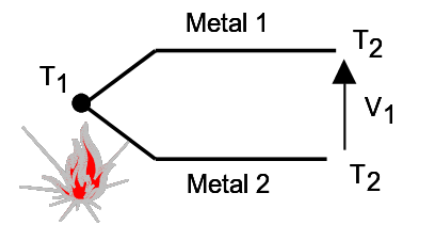
\includegraphics[scale=0.5]{./../images/termopar.png}
\caption{esquemáticos de um termopar}
\label{fig:termopar}
\end{figure}

\newpage

\section{Material}
Para a calibração usaremos;
\begin{itemize}
	\item 2 termopares. Chamamo-os: o SMP(sistema de mediçõa padrão) e o SMC(sistema de medição a calibrar)
	\item isopor com gelo fundente
	\item forno para banho maria com cabeça termostática
	\item multímetro digital
\end{itemize}
\section{Procedimentos}
\paragraph{}Inicialmente realizamos as conexões dos termopares ao multímetro digital. 
Pode ser útil utilizar dois multímetros para podermos ler simultâneamente as medidas
do SMP e do SMC. O termopar SMP utilizado fornece a saída em Ohms, enquanto o SMC em 
Volts. A conexão deve levar esses dois fatos em consideração para
que seja feita adequadamente. Para melhorar os resultados usamos uma conexão
com fios condutores de compensação.
A ponta fria de ambos os termopares são colocadas no isopor com gelo fundente e as pontas quentes são
colocadas no forno de banho maria com cabeça termostática.  As pontas ficarão
nessa configuração durante todo o experimento. Com o forno em temperatura ambiente
fazemos 4 leituras dos multímetros. As leituras são feitas com intervalos de 20 segundos
para padronização. O processo é refeito para 3 outras diferentes temperaturas do banho maria.
É importante notar que depois que configuramos a temperatura do forno é preciso esperar um
tempo para que esta seja atingida. 

\subsection{Dificuldades Encontradas}
\paragraph{}Inicialmente planejava-se realizar as três ultimas medidas nas temperaturas de
200º, 300º e 400ªC. Não foi possível atingir tais temperaturas pois o tempo que o forno
utilizado demoraria para atingí-las seria impraticavel. Utilizamos portanto temperatura
intermediárias. Para conhecermos as temperaturas que estávamos medindo utilizamos a tabela
de referência do temopar SRP. Essa tabela relaciona a resistência medida no multímetro
com a temperatura na ponta quente desde que a ponta fria esteja em 0ºC. 

\newpage

\section{Dados Experimentais}
\paragraph{}As tabelas a seguir foram obtidas:

\FloatBarrier
\begin{table}[!htp]
	\parbox{.45\linewidth}{
		\centering
		\begin{tabular}{|l|l|l|} \hline
			& SMP & SMC \\ \hline
			Pontos & Unidade[$\Omega$] & Unidade [mV]\\ \hline
			01&109.102 & 0.848 \\ \hline
			02&109.101 & 0.848\\ \hline
			03&109.100 & 0.849\\ \hline
			04&109.104 & 0.850\\ \hline
		\end{tabular}

		\caption{1ª temperatura}
		}
\hfill
	\parbox{.45\linewidth}{
		\centering
		\begin{tabular}{|l|l|l|} \hline
			& SMP & SMC \\ \hline
			Pontos & Unidade[$\Omega$] & Unidade [mV]\\ \hline
			01	&	171.64 & 6.838 \\ \hline
			02	&	171.73 & 6.864\\ \hline
			03	&	171.74 & 6.889\\ \hline
			04	&	171.81 & 6.906\\ \hline
		\end{tabular}

		\caption{2ª temperatura}
		}
\end{table}

\begin{table}[!htp]
	\parbox{.45\linewidth}{
		\centering
		\begin{tabular}{|l|l|l|} \hline
			& SMP & SMC \\ \hline
			Pontos & Unidade[$\Omega$] & Unidade [mV]\\ \hline
			01	& 200.47 & 10.923 \\ \hline
			02	& 200.73 & 10.950\\ \hline
			03	& 200.90 & 10.971\\ \hline
			04	& 200.45 & 10.991\\ \hline
		\end{tabular}

		\caption{3ª temperatura}
		}
\hfill
	\parbox{.45\linewidth}{
		\centering
		\begin{tabular}{|l|l|l|} \hline
			& SMP & SMC \\ \hline
			Pontos & Unidade[$\Omega$] & Unidade [mV]\\ \hline
			01	& 219.24 & 13.066 \\ \hline
			02	& 219.39 & 13.081\\ \hline
			03	& 219.43 & 13.093\\ \hline
			04	& 219.66 & 13.109\\ \hline
		\end{tabular}

		\caption{4ª temperatura}
		}
\end{table}
\FloatBarrier
\section{Análise de Dados}
\paragraph{} Dividimos a análise em seções para melhor entendimento.
\subsection{Questão 1}
\paragraph{}Calculamos $\overline{T}$ e $s_T^2$ pelas fórmulas:
	\begin{equation}
		\begin{array}{l}
		\overline{T} = \frac{\sum_{i = 1}^{n} T_i}{n} \\
		s_T^2 = \frac{\sum_{i = 1}^{n} (T_i - \overline{T})^2}{n(n-1)}
		\end{array}
	\end{equation}
	\paragraph{}Os resultados são mostrados na tabela a seguir.
\FloatBarrier
\begin{table}
		\centering
		\begin{tabular}{|l|l|l|l|} \hline
			Ponto(ºC)& $\overline{T}$ & $s_T^2$  & $s_T$ \\ \hline
			23		&       	0,84825	& 	6,25E-08		&0.000478714	\\ \hline
			188,5	& 		6,87425	&	2,20396E-04	&0.0148457	\\ \hline
			269   	&  		10,9595	& 	2,2875E-04	&	0.0151245\\ \hline
			321    	& 		13,08725&   8,30625E-05	&	0.00911386\\ \hline
		\end{tabular}
		\caption{média e desvio padrão para as medições}
		\label{tab:quest1}
\end{table}
\FloatBarrier
Os pontos foram tomados procurando a média dos valores medidos no SMP e 
procurando por essa media na tabela do fabricante.
\subsection{Questão 2}
\paragraph{} A curva de calibração é feita com os dados da tabela acima. A equação obtida por regressão linear
é:

\begin{equation}
	V(T) = 0.0413 T -0.3254
	\label{eq:regrec}
\end{equation}

O resultado grádico é plotado a seguir.
\FloatBarrier
\begin{figure}[!htp]
    \begin{subfigure}[!htp]{0.3\textwidth}
        % GNUPLOT: LaTeX picture with Postscript
\begingroup
  \makeatletter
  \providecommand\color[2][]{%
    \GenericError{(gnuplot) \space\space\space\@spaces}{%
      Package color not loaded in conjunction with
      terminal option `colourtext'%
    }{See the gnuplot documentation for explanation.%
    }{Either use 'blacktext' in gnuplot or load the package
      color.sty in LaTeX.}%
    \renewcommand\color[2][]{}%
  }%
  \providecommand\includegraphics[2][]{%
    \GenericError{(gnuplot) \space\space\space\@spaces}{%
      Package graphicx or graphics not loaded%
    }{See the gnuplot documentation for explanation.%
    }{The gnuplot epslatex terminal needs graphicx.sty or graphics.sty.}%
    \renewcommand\includegraphics[2][]{}%
  }%
  \providecommand\rotatebox[2]{#2}%
  \@ifundefined{ifGPcolor}{%
    \newif\ifGPcolor
    \GPcolorfalse
  }{}%
  \@ifundefined{ifGPblacktext}{%
    \newif\ifGPblacktext
    \GPblacktexttrue
  }{}%
  % define a \g@addto@macro without @ in the name:
  \let\gplgaddtomacro\g@addto@macro
  % define empty templates for all commands taking text:
  \gdef\gplbacktext{}%
  \gdef\gplfronttext{}%
  \makeatother
  \ifGPblacktext
    % no textcolor at all
    \def\colorrgb#1{}%
    \def\colorgray#1{}%
  \else
    % gray or color?
    \ifGPcolor
      \def\colorrgb#1{\color[rgb]{#1}}%
      \def\colorgray#1{\color[gray]{#1}}%
      \expandafter\def\csname LTw\endcsname{\color{white}}%
      \expandafter\def\csname LTb\endcsname{\color{black}}%
      \expandafter\def\csname LTa\endcsname{\color{black}}%
      \expandafter\def\csname LT0\endcsname{\color[rgb]{1,0,0}}%
      \expandafter\def\csname LT1\endcsname{\color[rgb]{0,1,0}}%
      \expandafter\def\csname LT2\endcsname{\color[rgb]{0,0,1}}%
      \expandafter\def\csname LT3\endcsname{\color[rgb]{1,0,1}}%
      \expandafter\def\csname LT4\endcsname{\color[rgb]{0,1,1}}%
      \expandafter\def\csname LT5\endcsname{\color[rgb]{1,1,0}}%
      \expandafter\def\csname LT6\endcsname{\color[rgb]{0,0,0}}%
      \expandafter\def\csname LT7\endcsname{\color[rgb]{1,0.3,0}}%
      \expandafter\def\csname LT8\endcsname{\color[rgb]{0.5,0.5,0.5}}%
    \else
      % gray
      \def\colorrgb#1{\color{black}}%
      \def\colorgray#1{\color[gray]{#1}}%
      \expandafter\def\csname LTw\endcsname{\color{white}}%
      \expandafter\def\csname LTb\endcsname{\color{black}}%
      \expandafter\def\csname LTa\endcsname{\color{black}}%
      \expandafter\def\csname LT0\endcsname{\color{black}}%
      \expandafter\def\csname LT1\endcsname{\color{black}}%
      \expandafter\def\csname LT2\endcsname{\color{black}}%
      \expandafter\def\csname LT3\endcsname{\color{black}}%
      \expandafter\def\csname LT4\endcsname{\color{black}}%
      \expandafter\def\csname LT5\endcsname{\color{black}}%
      \expandafter\def\csname LT6\endcsname{\color{black}}%
      \expandafter\def\csname LT7\endcsname{\color{black}}%
      \expandafter\def\csname LT8\endcsname{\color{black}}%
    \fi
  \fi
  \setlength{\unitlength}{0.0500bp}%
  \begin{picture}(7936.00,5668.00)%
    \gplgaddtomacro\gplbacktext{%
      \csname LTb\endcsname%
      \put(814,704){\makebox(0,0)[r]{\strut{} 0}}%
      \put(814,1319){\makebox(0,0)[r]{\strut{} 2}}%
      \put(814,1933){\makebox(0,0)[r]{\strut{} 4}}%
      \put(814,2548){\makebox(0,0)[r]{\strut{} 6}}%
      \put(814,3163){\makebox(0,0)[r]{\strut{} 8}}%
      \put(814,3778){\makebox(0,0)[r]{\strut{} 10}}%
      \put(814,4392){\makebox(0,0)[r]{\strut{} 12}}%
      \put(814,5007){\makebox(0,0)[r]{\strut{} 14}}%
      \put(946,484){\makebox(0,0){\strut{} 0}}%
      \put(1888,484){\makebox(0,0){\strut{} 50}}%
      \put(2830,484){\makebox(0,0){\strut{} 100}}%
      \put(3772,484){\makebox(0,0){\strut{} 150}}%
      \put(4713,484){\makebox(0,0){\strut{} 200}}%
      \put(5655,484){\makebox(0,0){\strut{} 250}}%
      \put(6597,484){\makebox(0,0){\strut{} 300}}%
      \put(7539,484){\makebox(0,0){\strut{} 350}}%
      \put(176,2855){\rotatebox{-270}{\makebox(0,0){\strut{}Voltagem V}}}%
      \put(4242,154){\makebox(0,0){\strut{}Temperatura(ºC)}}%
      \put(4242,5337){\makebox(0,0){\strut{}Calibração Estática de Termopar}}%
    }%
    \gplgaddtomacro\gplfronttext{%
      \csname LTb\endcsname%
      \put(6552,1097){\makebox(0,0)[r]{\strut{}data}}%
      \csname LTb\endcsname%
      \put(6552,877){\makebox(0,0)[r]{\strut{}regressão linear}}%
    }%
    \gplbacktext
    \put(0,0){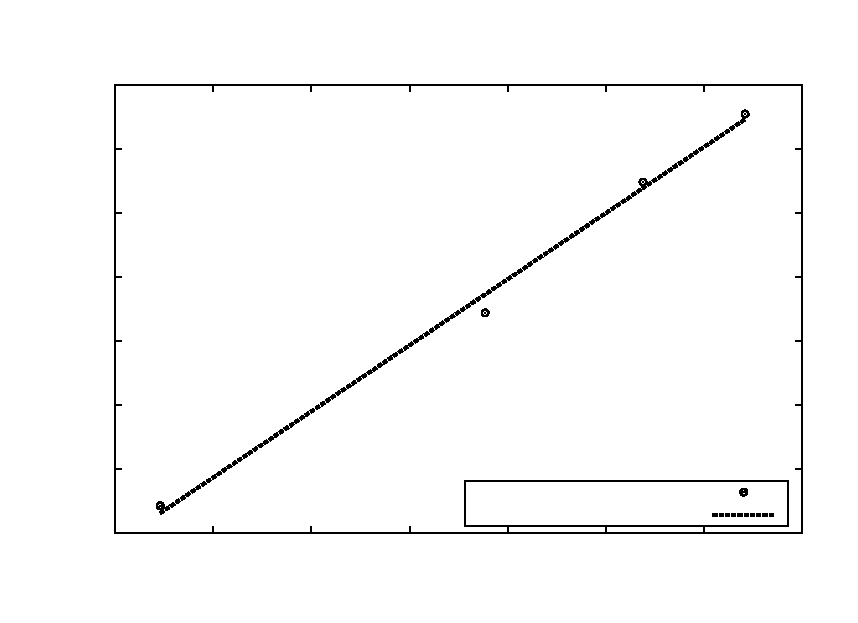
\includegraphics{graph-calibration}}%
    \gplfronttext
  \end{picture}%
\endgroup

        \caption{curva de calibração}
        \label{graph-1}  
    \end{subfigure}
\end{figure}
\FloatBarrier
\subsection{Questão 3}
\paragraph{} A equação \ref{eq:regrec} na questão 2 nos dá:
\begin{equation}
	\begin{array}{l}
	m = 0.0413 \\
	c = -0.3254
	\end{array}
	\label{qe:MeC}
\end{equation}

Podemos ir além e calcular a variação desses parâmetros. As fórmulas são:
\begin{equation}
	\begin{array}{l}
	s_m^2 = \frac{Ns_{q_o}^2}{N\sum q_i^2 - (\sum q_i)^2} \\
	s_b^2 = \frac{s_{q_o}^2 \sum q_i^2}{N\sum q_i^2 - (\sum q_i)^2}\\
	s_{q_o}^2 = \frac{1}{N} \sum (mq_i + b -q_o)^2	 \\
	s_{q_i}^2 = \frac{s_{q_o}^2}{m^2}
	\end{array}
\end{equation}

Onde $s_{q_o}$ nota o desvio padrão de $q_o$. Aqui $q_o$ são os valores de resposta à $q_i$ e assumimos que
o desvio de cada $q_o$ é igual, ou seja, que todas as medidas tem a mesma confiabilidade. Dessa forma $s_{q_o}$ é 
calculado usando informação de todos os pares $(q_i, q_o)$. Os índices \textbf{i} e \textbf{o} são para input e output. 
Os resultados são apresentados a seguir:

\FloatBarrier
\begin{table}[!htp]
		\centering
		\begin{tabular}{|l|l|} \hline
			Medida		& 			valor \\ \hline
			$S_{q_0}$	& 		0.33439	\\ \hline
			$S_m$			&       	0.0014827	\\ \hline
			$S_c$			&  		0.340911	\\ \hline
			$S_{q_i}$  	& 		2.84679 \\ \hline
		\end{tabular}
		\caption{média e desvio padrão para as medições}
\end{table}
\FloatBarrier

Vemos que existe relativamente grande incerteza em relação ao coeficiente
linear da reta, ao passo que baixa incerteza em relação ao coeficiente angular.


\subsection{Questão 4}
\paragraph{} Para efeito de comparação podemos calcular a soma das incertezas para cada ponto na tabela
\ref{tab:quest1} : 
	\begin{equation}
		\sum S_t = 0.0395628
	\end{equation}
	
	vemos que a incerteza $S_{q_o}$ tomada como uniforma para todos os pontos é muito maior que a
	soma das reais incertezas para cada ponto. Isso mostra que $S_{q_o}$ é uma cota superior para os
	valores reais de incerteza. Comparando com $S_m$ vemos que o erro no coeficiente angular da reta
	é inferior a soma dos erros individuais de cada medida. Ou seja, temos uma boa estimativa para
	o coeficiente angular da reta mesmo que os erros individuais de cada medida sejam altos.
\subsection{Questão 5}
\paragraph{} Os comentários pertinentes foram feitos ao longo dos itens anteriores.

\subsection{Questão 6}
	\paragraph{} Termistores não são nada mais nada menos que resistores termicamente sensíveis, isto é, são resistores que tem sua resistência alterada a medida que ocorre uma variação na sua temperatura. Essa variação da resistência em função da temperatura pode se dar em duas maneiras distintas, a primeira delas, à medida que a temperatura aumenta, a resistência do Termistor diminui, a esse tipo de termistor damos o nome de NTC. Já para o caso em que a resistência do termistor aumenta à medida que a temperatura sobe, damos a esse tipo de termistor o nome de PTC. É interessante notar que pequenas variações na temperatura, provocam grandes variações na resistência do termistor, essa relação costuma ser de natureza exponencial.
	\paragraph{}A diferença mor entre termistores e termoresistencias está em suas composições e processos de fabricação que são distintos. Enquanto que as termoresistencias são feitas de materiais condutores tais como a platina, o cobre ou o níquel, os termistores são compostos de misturas semicondutoras, como magnésio, cobalto, titanio...
	\paragraph{}As principais aplicações dos termistores encontram-se ligadas a funções como controle e compensação de variações de temperaturas nas faixas mais baixas. E em geral são utilizados numa faixa de temperaturas que vão de -100º à cerca de 300º. Por razões óbvias são várias vezes utilizados como sondas de temperaturas em ambientes industriais, aparelhagem médica, eletrodomesticos ou até mesmo na aparelhagem de investigações cientificas.
	\paragraph{}Outro ponto importante a falar sobre os termistores é a respeito de sua precisão. Em alguns casos, conseguimos verificar uma precisão da ordem de 1ºC na medição de temperatura, enquanto em outros casos, conseguimos verificar até mesmo a precisão de centésimos de grau.
	\paragraph{}Quando comparados com os termopares, conseguimos traçar tanto pra um quanto para o outro, vantagens e desvantagens em relação ao seu uso sobre o outro. De inicio podemos citar que termopares geram sua propria tensão, e logo não precisam ser alimentados por nenhuma corrente de excitação, em suma, podemos dizer que isso é uma vantagem para os termopares pois desse modo, evitamos o auto aquecimento que pode acontecer com os termistores ao serem alimentados, além disso, podemos citar que os termopares são simples, robustos, faceis de construir e operam numa ampla faixa de temperaturas. Agora que falamos das vantagens que o termopar leva sobre os termistores, veremos agora algumas desvantagens: Os termopares apresentam um baixo nivel da saída, apresentam uma caracteristica não linear e precisam de uma compensação da sua temperatura de junção de referencia.
\subsection{Questão 7}
\paragraph{}Desejamos aplicar o teste chi-quadrado para determinar se uma amostra de dados é gaussiana ou não.
Dividimos o procedimento em etapas. Essa questão levou ao desenvolvimento de um código em C++ para trabalhar
com os dados estatísticos, esse código está anexado ao final do relatório. Ele contém diversas rotinas para manipulação
de matrizes e dados estatísticos e utiliza somente as bibliotecas padrões da linguagem.

\begin{itemize}
\item \textbf{Ordenando os dados}
\paragraph{} O conjunto de dados é ordenado. Utiliza-se para isso um algoritmo simples implementado em C++. 
A ordenação não é mostrada aqui por ser de pouco interesse mas pode ser vista na tabela \ref{tan:grupos}
 onde definimos os grupos.

\item \textbf{Calculando Desvio Padrão e Média}
Novamente se utiliza rotinas em C++ para o calculo. Os resultados são:

\begin{equation}
	\begin{array}{l}
		\overline{x} = 9.83467 \\
		s = 0.428057 
	\end{array}
\end{equation}

\item \textbf{separando em grupos}
Os grupos são apresentados a seguir. Eles foram escolhidos de forma a termos no 
mínimo 5 elementos por grupo e a manter uma certa uniformidade no tamanho do intervalo.
\FloatBarrier
\begin{table}[!htp]
	\begin{tabular}{|l|} \hline
\textbf{grupo 1} \\ \hline
8.9 \\ \hline
8.99\\ \hline
8.99\\ \hline
9.06\\ \hline
9.2\\ \hline
	\end{tabular}
	\begin{tabular}{|l|} \hline
\textbf{grupo 2}\\ \hline
9.36\\ \hline
9.38\\ \hline
9.79\\ \hline
9.81\\ \hline
9.86 \\ \hline
9.87\\ \hline
9.89\\ \hline
9.9\\ \hline

	\end{tabular}
	\begin{tabular}{|l|} \hline
\textbf{grupo 3}\\ \hline
9.98\\ \hline
10\\ \hline
10.01\\ \hline
10.02\\ \hline
10.07\\ \hline
10.1\\ \hline
10.1\\ \hline
10.1\\ \hline
10.1\\ \hline
10.1\\ \hline
10.1\\ \hline
	\end{tabular}
	\begin{tabular}{|l|} \hline
\textbf{grupo 4}\\ \hline
10.11\\ \hline
10.15\\ \hline
10.2\\ \hline
10.2\\ \hline
10.32\\ \hline
10.38\\ \hline
	\end{tabular}
	\caption{grupos formados}
	\label{tan:grupos}
\end{table}
\FloatBarrier
\item \textbf{definir os limites dos intervalos e a respectiva normalização}
A normalização é feita pela fórmula:
	\begin{equation}
		w = \frac{x - \mu }{\sigma}
	\end{equation}
	onde devemos fazer a normalização nos extremos do intervalo. A tabela a seguir é montada:
\FloatBarrier	
	\begin{table}[!htp]
	\centering
	\begin{tabular}{|l|l|l|l|} \hline
	número do grupo & domínio em x & domínio em w & $n_o$ \\ \hline
1	 & -$\infty$ <x $\leq$ 9.2 & $-\infty$< w $\leq$-1.48267 & 5\\ \hline
2	&  9.2<x	$\leq$ 9.9 &  -1.48267< w $\leq$0.152628 & 8\\ \hline
3	&  9.9<x $\leq$ 10.1 & 0.152628< w $\leq$0.619855 & 11\\ \hline
4	&  10.1<x $< \infty$  & 0.619855< w < $\infty$ & 6\\ \hline

	\end{tabular}
	\end{table}
	
\FloatBarrier
	\item \textbf{Calculamos o número $n_e$ para cada intervalo} 
	Para cada intervalo calculamos o número de elementos que um ensaio com 30 tomadas teria de uma gaussiana
	perfeita.
	\FloatBarrier
	\begin{table}[!htp]
	\centering
	\begin{tabular}{|l|l|l|} \hline
	número do grupo & probabilidade & 30*probabilidade \\ \hline
1	 & 0.0690812 & 2.07244  \\ \hline
2	 &0.491573 & 14.7472\\ \hline
3	 &0.171669 & 5.15008\\ \hline
4	 &0.267676 &8.03029 \\ \hline
	\end{tabular}
	\end{table}
	 \FloatBarrier
	 
	 O cálculo da probabilidade foi feito utilizando uma aproximação numérica para a função de distribuição acumulada
	 gaussiana. O código pode ser visto em anexo.

\item Calculamos o fator $\chi^2$
dado pela fórmula:
	\begin{equation}
		\chi^2 = \sum _{i = i}^n \frac{(n_0 - n_e)^2}{n_e^2}
	\end{equation}

\begin{enumerate}
	\item	$n_e$ : número de elementos obtidos em um ensaio gaussiano perfeito para aquele intervalo
	\item $n_o$ números de elementos no grupo
\end{enumerate}

O fator calculado é :
\begin{equation}
	\chi^2 = 14.3807
\end{equation}

Agora, temos 4 grupos portanto apenas 1 grau de liberdade. Para 1 grau de liberdade, se tivéssemos obtido um
$\chi^2$ de 2.71 teríamos apenas 10\% de chance de termos uma gaussiana perfeita. Portanto temos menos de 10\%
de chances de ter uma gaussiana perfeita. O teste nos diz que \textbf{a distribuição não é gaussiana}!

\end{itemize}
\newpage

\section{Conclusão}
\paragraph{} O experimento permitiu obter a curva de calibração de um termopar. A curva achada foi 	V(T) = 0.0413 T -0.3254. Além disso obteve-se os diversos parâmetros associados a confiabilidade desses valores. Obteve-se que apesar
de certa incerteza na medição dos pontos individuais têm-se uma grande certeza do coeficiente angular obtido. 
Pôde-se também aplicar o teste chi-quadrado para uma amostra de 30 dados e determinar que esta não é
gaussiana. O experimento colocou em prática diversos conceitos de calibração e estatística e mostra como
essas técnicas são utilizadas na prática de engenharia.



\begin{thebibliography}{1}

\bibitem{sisMed}
Ernest D. Doebelin, \emph{Measurement Systems : application and design}, 3ª ed. McGraw Hill, 1993. 
\end{thebibliography}

\end{document}


